\documentclass[math,code]{amznotes}
\setcounter{tocdepth}{2}  % Only show subsections and sections in the ToC
\usepackage[utf8]{inputenc}
\usepackage{amsmath}
\usepackage{amsfonts}
\usepackage{graphicx}
\usepackage{tikz}
\usepackage{etoolbox}
\usepackage{tabularx}
\usepackage{float} % Needed for [H] placement specifier
\usepackage{wrapfig} % Needed for wrapping figures
\usepackage{diagbox} % For diagonal split in table
\usepackage{booktabs} % For better table formatting

\graphicspath{ {./images/} }
\geometry{
    a4paper,
    headheight = 1.5cm
}

\patchcmd{\chapter}{\thispagestyle{plain}}{\thispagestyle{fancy}}{}{}

\theoremstyle{remark}
\newtheorem*{claim}{Claim}
\newtheorem*{remark}{Remark}
\newtheorem{case}{Case}

\begin{document}
\fancyhead[L]{
    Design Thinking
}
\fancyhead[R]{
    Lecture Notes
}
\tableofcontents

\chapter{Empathize}
\section{Lecture Videos}
\subsection{An Introduction to Training your Empathy Muscle}
\begin{dfnbox}{Empathy}{dtn-empathy}
    {\color{red} \textbf{Empathy}} means stepping into someone else's shoes and experience the situation as they do.
\end{dfnbox}
One thing worth noting down is that, \textbf{Sympathy} and \textbf{Empathy} are different.
\begin{enumerate}
    \item \textbf{Sympathy} is a reaction to a struggle of other people. We feel bad about their situation, but by doing so, it sets a distance between us and them.
    \item \textbf{Empathy} is that we feel with other people. We are are willing to participate in their situation and experience what they are experiencing.
\end{enumerate}
To train our empathy, we can use the following two methods:
\begin{enumerate}
    \item In-depth interview
    \item Field observation
\end{enumerate}

\subsection{Context Mapping}
To do the context mapping, mainly consider the following 5 aspects, which will form your initial frame,
\begin{enumerate}
    \item \textbf{People}: Who are related? Who are involved? In this section, you will need to write whom you think as immediate users close to the frame. Then in an outer layer, identify groups of people whom your immediate users interact with, or who influence your immediate users.
    \item \textbf{Activities}: What chores? What do people do? This will determine the activities and actions of people you want to observe.
    \item \textbf{Place}: Where do these activities take place?
    \item \textbf{Time}: It can be the time of the day that the activity takes place. Or, it can be related to sequence. e.g., a time when the user comes from the outside or a time after it rains. Frequency can be considered too.
    \item \textbf{Issues}: What do you think are problems or difficulties? What might make problems? What do you need to know?
\end{enumerate}
These context mapping will prepare you for the questions you gonna to ask in the interview.

\subsubsection{My Context Mapping}
\begin{enumerate}
    \item \textbf{Initial Frame}: Taking care of plants
    \item \textbf{People}: A NUS student, his roommate (who he lives with) and his parents (where he gets money to buy things necessary for plants?)
    \item \textbf{Activities}: Water his plants and give plant vitamins. Put the plant somewhere to give the plants sunlight. When feeling boring alone in the room, what he will do to his plants? 
    \item \textbf{Place}: In his room. Bathroom (to get water), and outside to get vitamins. Balcony to get the sunlight.
    \item \textbf{Time}: Water his plant and give vitamins in the morning. How often does he do this? What happen if outside to travel and nobody cares about the plant?
    \item \textbf{Issues}: Cannot control how much water to give. Feel lonely. Busy schedule makes it difficult to give plants water as scheduled.
\end{enumerate}

After finishing the context mapping, the next thing you should do is to \textbf{select your interviewees}. You can interview the immediate user and the related user, but keep the number of users to be interviewed within 3.
\begin{notebox}
    \begin{remark}
        In this ILA, we will only focus on 1 user.
    \end{remark}
\end{notebox}

\subsection{In-depth Interview}
Below is an example of the flow of the interview,
\begin{enumerate}
    \item Introduce yourself and the project.
    \item Background information (if you don't have the user's profile)
    \item Factual information, e.g., past experience and process
    \item Motivation
    \item Preferences and opinions
    \item Challenges and future wishes
    \item Wrap-up the interview
\end{enumerate}
Here are some tips when conducting your interview
\begin{enumerate}
    \item Think your user as ``Experts of their lives'', and try to learn from them
    \item Avoid ``yes/no'' questions
    \item Ask open questions
    \item No leading questions
    \item No Jargons
    \item Prepare probing questions
    \item Ask ``Why''
\end{enumerate}

Before making the interview questions, think about what the \textbf{goal} of your interview will be!

\subsubsection{My practice for the power of 5 times ``Why''}
\textbf{For Watering Issues:}
\begin{itemize}
    \item ``Why does the water leak out from the pot?'' $\rightarrow$ ``I often overwater them.''
    \item \textit{1st Why}: ``\textbf{Why} does this happen?'' $\rightarrow$ ``I don’t know how much water they need.''
    \item \textit{2nd Why}: ``\textbf{Why} haven’t you looked up guidelines?'' $\rightarrow$ ``The instructions were confusing.''
    \item \textit{3rd Why}: ``\textbf{Why} were they confusing?'' $\rightarrow$ ``Terms like ‘soil porosity’ overwhelmed me.''
    \item \textit{4th Why}: ``\textbf{Why} does terminology stop you?'' $\rightarrow$ ``I fear killing the plants if I make mistakes.''
\end{itemize}

\subsubsection{My Interview Flow}
\begin{enumerate}
    \item \textbf{Introduction}
    \begin{itemize}
        \item ``Hi [Name], thank you for joining! My name is [Your Name], and I’m exploring how students like you integrate plant care into daily life. This will help design solutions for plant enthusiasts. The conversation will take about 30 minutes. Are you comfortable starting?''
    \end{itemize}
    
    \item \textbf{Background Information}
    \begin{itemize}
        \item ``Could you share about yourself? For example, your year of study or hobbies?''
        \item ``How did you first get interested in having plants in your room?''
        \begin{itemize}
            \item \textit{Probe}: ``What inspired you to start caring for plants?''
        \end{itemize}
    \end{itemize}
    
    \item \textbf{Factual Information (Routine \& Process)}
    \begin{itemize}
        \item ``Walk me through a typical day caring for your plants. What steps do you take?''
        \begin{itemize}
            \item \textit{Probe}: ``Why do you water them at specific times?''
            \item \textit{Probe (1st Why)}: ``\textbf{Why} is controlling water amounts challenging?''
            \item \textit{Probe (2nd Why)}: ``\textbf{Why} does [previous answer] make measuring hard?''
            \item \textit{Probe (3rd Why)}: ``\textbf{Why} haven’t you tried tools to address this?''
        \end{itemize}
        \item ``Where do you get plant supplies like vitamins? How do you decide what to buy?''
        \item ``Have you ever traveled and left your plants unattended? What happened?''
        \begin{itemize}
            \item \textit{Probe (1st Why)}: ``\textbf{Why} is [e.g., ‘plants dying’] a concern?''
            \item \textit{Probe (2nd Why)}: ``\textbf{Why} don’t you ask others for help?''
        \end{itemize}
    \end{itemize}
    
    \item \textbf{Motivation (Emotional Connection)}
    \begin{itemize}
        \item ``What do you enjoy most about having plants?''
        \begin{itemize}
            \item \textit{Probe (1st Why)}: ``\textbf{Why} is [e.g., ‘calmness’] important to you?''
            \item \textit{Probe (2nd Why)}: ``\textbf{Why} do plants help you feel that way?''
        \end{itemize}
        \item ``What keeps you motivated to care for plants when busy?''
    \end{itemize}
    
    \item \textbf{Preferences \& Opinions (Interactions \& Ideal Setup)}
    \begin{itemize}
        \item ``When bored or lonely, how do your plants affect your mood?''
        \begin{itemize}
            \item \textit{Probe}: ``Describe a time plants changed your emotions.''
        \end{itemize}
        \item ``If you could design the perfect plant environment, what would it look like?''
        \begin{itemize}
            \item \textit{Probe (1st Why)}: ``\textbf{Why} is [feature] important to you?''
        \end{itemize}
    \end{itemize}
    
    \item \textbf{Challenges \& Future Wishes (Root Cause Analysis)}
    \begin{itemize}
        \item \textbf{Watering Issues}:
        \begin{itemize}
            \item ``Can you describe a time over/underwatering caused problems?''
            \item \textit{Probe (1st Why)}: ``\textbf{Why} do you think that happened?''
            \item \textit{Probe (2nd Why)}: ``\textbf{Why} didn’t you notice earlier?''
            \item \textit{Probe (3rd Why)}: ``\textbf{Why} is tracking plant condition hard?''
        \end{itemize}
        \item \textbf{Loneliness}:
        \begin{itemize}
            \item ``How do plants help when you feel lonely?''
            \item \textit{Probe (1st Why)}: ``\textbf{Why} do you turn to plants over people?''
            \item \textit{Probe (2nd Why)}: ``\textbf{Why} is this companionship meaningful?''
        \end{itemize}
        \item \textbf{Travel Disruptions}:
        \begin{itemize}
            \item ``What worries you most about leaving plants during travel?''
            \item \textit{Probe (1st Why)}: ``\textbf{Why} is [answer] a concern?''
            \item \textit{Probe (2nd Why)}: ``\textbf{Why} don’t you trust others to help?''
        \end{itemize}
        \item ``If you could solve one plant-related problem magically, what would it be?''
    \end{itemize}
    
    \item \textbf{Wrap-Up}
    \begin{itemize}
        \item ``Is there anything we haven’t discussed that you’d like to share?''
        \item ``Thank you! Your insights are invaluable. Would you like project updates?''
    \end{itemize}
\end{enumerate}

\subsection{Field Observation}
Here are some tips when doing field observation
\begin{enumerate}
    \item Take photos or note observations down quickly on your notebook (Get permission from your user)
\end{enumerate}

\subsection{Individual Learning Activity}
Basically, this ILA should follow the steps below
\begin{enumerate}
    \item \textbf{User Journey Map}: Basically, this step asks you to divide your observation into several stages. And among each stage, record the user's feeling/emotion.
    \item \textbf{Key Findings}: These findings should come from your user journey map. Note that add more visuals!
    \item \textbf{Reframe Design Challenge}: think about how you frame your design challenge differently given your latest insights into user behavior, motivation, goals and challenges.
    \item \textbf{Reiterate Idea}: Use what you have been trained for during Segment 1 and the field study you have conducted during this segment, and then come up with a modified or new idea that will work best to help your specific user. Note that you should also include the visual and the idea in this step will likely be the final one you are going to implement in the future!
    \item \textbf{Reflection}: As usual. Can use the Bloom's Taxonomy to structure your reflection. So basically, bloom's taxonomy is to
    \begin{itemize}
        \item Describe what you have done. (This is called \textbf{Remember and Understand})
        \item Then think about how to apply them in DT. (This is called \textbf{Apply})
        \item Eventually think about how you can evaluate, analyze and create new knowledge with it. (This is called \textbf{creating, evaluating and creating})
    \end{itemize}
\end{enumerate}

\section{Individual Learning Activity}
\subsection{User Journey Map}
My user is \textbf{George, 19 years old, SoC undergraduate} who wants to \textbf{water his plants efficiently, maximizing water use while avoiding runoff and cleanup.}
\begin{enumerate}
    \item \textbf{Fetch Water}:
    \begin{itemize}
        \item \textbf{Action}: Slowly fill a plastic cup (the watering tool) with water from the washroom faucet.
        \item \textbf{Emotion}: Cheerful and motivated, imagining how the plant will thrive after watering.
        \item \textbf{Pain Points}: Limited by the size of the watering tool, it is difficult to control how much water to fill in the cup.
    \end{itemize}
    \item \textbf{Carry water from washroom to plant}:
    \begin{itemize}
        \item \textbf{Action}: Carefully transport the filled cup to the plant’s location to avoid spilling.
        \item \textbf{Emotion}: Mildly annoyed because some water spilled on the way, but trying to keep happy (from the picture)
        \item \textbf{Pain Points}: Since the cup lacks a cover, water may spill during transport, adding extra cleaning effort later.
    \end{itemize}
    \item \textbf{Water the plant}
    \begin{itemize}
        \item \textbf{Action}: Identify a suitable spot near the plant and pour the water gently onto the soil.
        \item \textbf{Emotion}: Slightly frustrated and impatient because the pot is too small, making it hard to find a good spot to pour the water.
        \item \textbf{Pain Points}: The plant's leaves cover most of the soil's surface, making it hard to find a spot to pour water evenly onto the soil.
    \end{itemize}
    \item \textbf{Refill the watering tool}
    \begin{itemize}
        \item \textbf{Action}: Upon realizing more water is needed, return to the washroom, refill the cup, and continue watering.
        \item \textbf{Emotion}: A bit irritated because realizing there isn’t enough water means having to go back and repeat the process.
        \item \textbf{Pain Points}: Initially unsure of how much water the plant needs, and limited by the watering tool's size, requiring multiple trips to refill.
    \end{itemize}
    \item \textbf{Clean up excess water}
    \begin{itemize}
        \item \textbf{Action}: Use a rag or some tissues to wipe up any spilled water and ensure the surrounding area remains dry.
        \item \textbf{Emotion}: Relieved but slightly annoyed because the watering is finally done, but cleaning up of the excess water is still necessary.
        \item \textbf{Pain Points}: After watering, not only is there excess water spilled from the plant, but there is also leftover water in the watering tool that needs to be dealt with.
    \end{itemize}
\end{enumerate}

\subsection{Key Findings}
\begin{enumerate}
    \item \textbf{Watering a plant requires an important prerequisite: an ``empty'' space where the water can be poured to the plant.} \\
    In my field study, the first key finding I discovered was where to water the plant. Since the plant is in a pot, its body and leaves may cover most of the surface of the pot. This creates a challenge when watering, as when we use traditional watering, the water is more likely to run off the leaves and spill over the sides of the pot, preventing it from reaching the soil. Furthermore, if a traditional watering tool, like a plastic cup, is used, it becomes even harder to water the plant effectively. This is because we cannot easily position the cup through the leaves to pour water directly onto the soil. In some cases, where the plant’s leaves are more spread out, it’s possible to gently move them aside by hand to water. However, for my user’s succulent plant, the leaves are densely packed, making it difficult to water without the water flowing off the leaves.
    \item \textbf{After watering, it's necessary to clean up not only the water that has spilled from the plant, but also the excess water in the watering tool.} \\
    My second key finding was that: after watering the plant, it's not just the water that runs out of the pot that needs to be cleaned up, but also the remaining water in the watering tool needs to be dealt properly. During my field study, I discovered that my interviewee also faced the issue of dealing with the excess water left in the watering tool. He thought that simply discarding it seemed wasteful, and leaving it somewhere felt a bit awkward. As a result, I realized that after watering, it’s necessary to clean up not just the water spilled from the plant, but also the extra water remaining in the watering tool, this is what I have never thought of initially.
\end{enumerate}

\subsection{Reframe Design Challenge}
The part is recommended to use the \textbf{Venn Diagram}.
\begin{enumerate}
    \item \textbf{Important takeaways}:
    \begin{itemize}
        \item \textbf{Segment 1}: Taking care of plants requires providing the right and proper amount of water, which can be a cumbersome and inefficient process.
        \item \textbf{Segment 2}: My user loves simplicity and ease of use, and he doesn't want to waste anything. Particularly, he has a strong pursuit for maximizing the use of resources.
        \item \textbf{Overlapped part}: I plan to approach my design challenge by creating a simple, user-friendly and multifunctional ``pipe system'' that integrates plant care, watering, and nutrient supply, allowing my user to take care of his plants more easily and enjoy the process of taking care of plants.
    \end{itemize}
    \item \textbf{Re-framed Design Challenge}:
    \begin{itemize}
        \item \textbf{How might I help}: my friend George
        \item \textbf{achieve ways to}: water his plants properly and efficiently
        \item \textbf{considering}: that his plant’s leaves may obstruct direct access to the soil and his strong preference for simplicity and ease of use.
    \end{itemize}
\end{enumerate}

\subsection{Iterate on the Idea}
This part is mainly done on the draw.io, using the flowchart diagram to illustrate the iteration flow.

\subsection{Reflection}
From observing people in their context, I learned that Design Thinking is to have deep empathy to the guest (a.k.a my user) at the start of any problem.

In the lecture, I learned that empathy means stepping into someone else’s shoes and experiencing the situation as they do. I discovered that the primary benefit of empathy in my design challenge was its ability to help me focus on the specific problem I needed to solve. The lecture also emphasized that sympathy and empathy are not the same. While sympathy is merely a reaction to another person’s struggle, empathy involves truly feeling with them. I found that only by experiencing my user’s situation firsthand did I gain a deeper understanding of the problem I am going to solve. Below, I will explain how empathy has guided me through the iterative process of refining my design challenge.

The lecture introduced several methods for practicing empathy, including context mapping, in-depth interviews, and field observations. In my context mapping exercise, guided by Prof. JJ, I considered who my potential users might be, what activities they engage in, where these activities occur, and at what times (see Figure 1). This exercise served as the first step in developing empathy and directed the focus of my subsequent field observations and in-depth interviews. For example, after completing the context mapping, I realized that I needed to pay particular attention to my user’s watering habits.

During the design and execution of the in-depth interviews, I was particularly struck by the ``power of 5 times why'' technique, which is to continuously ask ``why'' to move beyond surface issues and uncover the root causes. For example, as illustrated in Figure 2, I learned that while the immediate reason for overwatering was a lack of knowledge about the appropriate amount of water for plants, the deeper underlying issue was the user's fear that excessive water might kill the plants. This questioning process not only provided insights into the users’ personalities but also enabled me to explore and understand the underlying problems more thoroughly.

Then the field observation is, in my view, the most critical component of empathy. All the theoretical work must eventually be practiced in the real world. We may have heard the example of UberEATS. In UberEATS, the designers immerse themselves in local markets, experience the food culture firsthand, and observe how people interact with their designs.  My field observation was no exception, and as I conducted my field observation, I discovered many aspects that I had not thought of at all before. In the following, I would like to discuss what I have learned about design thinking from four aspects: dividing, analyzing and discovering insights, reframing the design challenge and optimizing my solution through iteration.

First of all, as mentioned in the lecture, during field observation, we will be faced with tons of information, and in most cases, there is no way for us to analyze every aspect of the matter right away. Therefore, in field observation, I think it is very important to record the important moments with photos. But how to determine which moment is important? In my opinion, this requires prior planning, i.e., dividing. for example, before field observation, I would divide observation into three parts, i.e., before watering, during watering and after watering. This idea is actually similar to dividing a big project into several manageable subproblems, then we solve each of the subproblems , and then we summarize the answers of these subproblems together to solve a big problem. To be honest, I practiced this thinking in my coding course, but I found that it can be put to good use in design thinking as well!

Once the field observations were completed, I analyzed each stage of the user journey map to identify insights. What is an insight? An insight is nothing but a revelation that is hidden in plain sight. To try to find insight, I start by recording the user’s emotions and identifying pain points at each stage, which is similar to finding the ``sucks'' statements! I realized that many innovations stem from dissatisfaction with existing conditions, which is what I learned in Segment 1! Immersing myself in the user’s experience led me to discover several issues I had not anticipated. For me, I mainly found two interesting insights: firstly, solving the watering problem required not only knowing the right amount of water but also ensuring there was ``enough space'' for us to water the plants; and second, not only the excess water leaking from the bottom of the pot needs to be managed, the excess water from the watering tool also needed to be managed. These insights greatly influenced and inspired my final design solution.

After gathering insights from both field observations and interviews, I gained a comprehensive understanding of the user’s needs and personality. This allowed me to reframe my design challenge with a clear focus, eliminating the initial confusion caused by having too many ideas in the Segment 1. I came to realize again that ``Design Thinking is to have deep empathy to the guest (a.k.a my user) at the start of any problem.''

To refine my solution, I adopted Professor Clayton Christensen’s Job To Be Done (JTBD) approach, which focuses on understanding the underlying motivations that lead customers to ``hire'' a product or service to accomplish a specific task. In the context of design thinking, the JTBD approach helped me ensure that my solution was centered around solving genuine customer problems. I started by listing all the jobs to be done and then iteratively refined my initial solution using techniques learned in the segment 1, such as making shifts and resonant pivots. After more than five rounds of iteration, I finally experienced a Eureka moment, capturing the essence of design thinking.

This entire process has reaffirmed for me that empathy is the cornerstone of design thinking. By deeply experiencing the user’s situation, breaking down a complex problem into manageable parts, uncovering critical insights, and continuously refining the solution, I have praticed a skill set which I think is essential for dealing with many big problems I may face in the future, as an Engineer. Design thinking, at its core, is about having deep empathy for the user from the very beginning of any problem-solving journey!

\section{Supplementary Readings}
\subsection{Insight}
\begin{dfnbox}{Insight}{dfn-insight}
    {\color{red} Insight} is a \textbf{revelation} that is hidden in plain sight.
\end{dfnbox}
\begin{exbox}{An Example for Insight}{example-insight}
    TikTok algorithm is known for its accuracy, but what if on your TikTok first page, sometimes you still get the disgusting videos? \\
    \textbf{Possible Insight}: We think the algorithms influence for the worse, but what if the algorithms just reveal the worst \textbf{of us}.
\end{exbox}

\subsection{Observation}
Sometimes, you don't have to ask questions to know a person better. Triangulate different observations together also helps!

This observation is meant to \textbf{know your user better}, thus you can reframe your design challenge according to your understanding of the user.

\subsection{Reframe your Design Challenge}
You can use the \textbf{H}ow \textbf{M}ight \textbf{W}e (HMW) statement to frame the design challenge on the right problems better.

The structure is,
\begin{enumerate}
    \item \textbf{How might we} + intended action
    \item \textbf{for} + primary user
    \item \textbf{so that} + desired outcome
\end{enumerate}
The \textbf{HMW} statement should not be too specific and too general.

\subsection{Case Study}
\subsubsection{Design Thinking (DT)}
Design Thinking (DT) is to have deep \textbf{empathy} for the \textbf{guest} at the start of any problem.

\subsubsection{JTBD Approach}
JTBD stands for ``Job To Be Done''. This approach is initiated by Prof Clayton Christensen, which focuses on understanding \textbf{the underlying needs and motivations} that drive customers to ``hire'' a product or service to accomplish a specific task or goal.

In Design Thinking, JTBD can be used to improve a product by ensuring that the design process is centered around solving real customer problems. By identifying the key ``job'' the user needs to get done, teams can:
\begin{enumerate}
    \item \textbf{Empathize More Deeply}: Understand users’ motivations beyond surface-level needs.
    \item \textbf{Ideate Effectively}: Generate solutions that directly address these jobs rather than just adding features.
    \item \textbf{Prototype \& Test Meaningfully}: Ensure solutions align with the job users are trying to accomplish.
\end{enumerate}

\subsubsection{UberEATS}
UberEATS immerses in local markets to understand customer needs. Their designers will go to different cities, move about the city, experience the food culture, and watch how people use the things we’ve designed.

\chapter{Do, Undo, Redo}
\section{Lecture Videos}
\subsection{An Introduction to Prototypes}
\begin{dfnbox}{Protytpe}{dfn-prototype}
    {\color{red} \textbf{Prototypes}} are objects that we make to mainfest our internal ideas.
\end{dfnbox}
\textbf{Prototypes} can serve as a mirror with which designers can use to reflect and access their internal understanding of a design situation. It deconstructs a complex design opportunity into smaller, manageable design issues. 

Donald Schoen, a researcher, called \textbf{prototyping} an iterative process of moving and seeing.
\subsection{The Types of Prototypes}
\begin{enumerate}
    \item Specific prototype: It focuses on \textbf{one design feature}.
    \item Comprehensive prototype: It attempts to address the whole system -- The ``Big Picture''.
    \item Low Fidelity prototype: It emphasizes \textbf{quantity and economy} over quality.
    \item High Fidelity prototype: It emphasize \textbf{quality and refinement}.
\end{enumerate}
\subsubsection{Some tips about prototype}
\begin{enumerate}
    \item Know why you are building a prototype: Making a prototype should shed light about the design situation that you find yourself in.
    \item Prototype appropriately: break down the problems into manageable chunks, don't need to solve all challenges in one prototype.
    \item Record the prototypes: Revisit your ideas often to try finding new insights.
\end{enumerate}

\subsection{Low Fidelity Prototyping}
In this part, we will introduce some techniques about how to quickly do the low fidelity prototyping.
\subsubsection{Techniques for easy prototypes}
\begin{enumerate}
    \item \textbf{Sketches}
    \item \textbf{Mockups}: They are a more polished rendering of a specific aspect of an idea. e.g., 3-D modelling. Mockups are about \textbf{how an idea looks like}
    \item \textbf{Simulations}: They are about \textbf{how an idea feels like and acts like}.
\end{enumerate}
\subsubsection{Techniques for comprehensive prototypes}
\begin{enumerate}
    \item \textbf{Paper prototypes}
    \item \textbf{Cardboard prototypes}
    \item \textbf{Wizard of Oz prototypes}: This refers to a prototyping technique where a user interacts with a system that appears to function autonomously, but in reality, a human is controlling part or all of its operations behind the scenes. This is often used in usability testing to simulate advanced AI or automation before full implementation.
\end{enumerate}

\subsection{Designerly Attitudes of Prototyping}
\subsubsection{Some Useful Tips}
\begin{enumerate}
    \item Prototyping is a lot about \textbf{making and making do}: This means that we should keep the \textbf{primary goal} of that prototype in mind and don't be distracted by polishing every other secondary detail.
    \item Prototyping is about \textbf{learning through doing, repeatedly}
    \item Prototyping is \textbf{not about doing the same thing over and over again}, rather \textbf{we reflect and learn from each prototype we build}
    \item Prototyping is \textbf{economy of means}: This means we should aim to be economical with all the prototypes that we build. 
    \item Prototypes are \textbf{objective objects}: This means we should take the comments and critique that our prototypes might receive positively and constructively.
\end{enumerate}

\subsection{Individual Learning Activity}
The workflow for this ILA is
\begin{enumerate}
    \item Combine ideas from Segment 1 and Segment 2
    \item Planning: This is about what you want to do with your prototype, 
    \item Building: Write a documentation
    \item Reflecting: As usual
\end{enumerate}

\section{Individual Learning Activity}
\subsection{My Prototype Agenda}
\begin{enumerate}
    \item \textbf{Pipe System}:
    The whole idea is to use \textbf{one straw only}, and remain the water to be poured as the same. Then by changing the design, record to time it takes for the same plant to absorb the the same amount of water.
    \begin{itemize}
        \item The original straw with no other holes.
        \item Dig some holes at the bottom, which should be buried in the soil. (Issue here, can the whole soil be watered?)
        \item Dig one hole above the soil, but not too high. (Not enough)
        \item Dig more holes around the same height. 
    \end{itemize}
    Issues arrived, I still need to pour the water manually! So, how about we add a container to store the water temporarily.
    \item \textbf{Water Tank}
    \begin{itemize}
        \item Make the top of the straw is at the same height with the bottom of the container. (No switch, too tall, not stable)
        \item Raise the height of the straw to implement an easy switch mechanism instead of using a valve! (More stable now!)
    \end{itemize}
\end{enumerate}
\subsection{Contextualize your Idea}
This part should be based on the segment 2 if you are not going to change your idea.
\begin{enumerate}
    \item \textbf{The key issue I want to tackle}: My user’s watering method (or the watering can) is not very efficient, and it is reflected in the following two aspects:
    \begin{itemize}
        \item Since the plant's leaves cover most of the soil, my user struggles to find an area that is empty enough for watering.
        \item After watering, my user notices that there is still some water left in the watering can and is unsure how to dispose of it properly.
    \end{itemize}
    \item \textbf{My insights on this issue}:
    \begin{itemize}
        \item Most of the time, we take it for granted that we can find an empty enough space for watering. However, for certain plants, finding such a space is not particularly easy.
        \item When it comes to handling excess water, we usually think of the water that drains from the plant’s pot. However, properly dealing with the leftover water in the watering can is not always easy either.
    \end{itemize}
    \item \textbf{My proposed idea is}: Create an efficient watering can, which mainly has the following three features.
    \begin{itemize}
        \item Removable, top-mounted water tank: It allows easy refilling (removable) and maintains a steady water supply (large enough so that refill once can ensure the plant gets enough water).
        \item A switch mechanism: it is located between the water tank and the three pipes, allowing water to flow immediately when opened and stop instantly when closed. 
        \item Three pipes system: Three pipes are used to deliver the water from the water tank to the soil. Organized in the triangle form to ensure the stability of the whole system as the triangle is considered the most stable and simplest shape.
    \end{itemize}
\end{enumerate}
\subsection{Plan your prototype}
\begin{enumerate}
    \item \textbf{What I want to learn about my idea with this prototype}: I want to test whether this watering can using the pipe system is efficient and stable enough. (By ``efficient'', I mean how quickly the soil can absorb the water. By ``stable'', I mean whether the system can stand firmly on the ground without being easily blown over by the wind.)
    \item \textbf{How I will build this prototype}: Mainly I will use the physical 3D mock-up and simulation to build-up my prototype. \textbf{Notes}: I will need the following materials
    \begin{itemize}
        \item A plastic box to serve as a container
        \item Some straws to sour as the pipe
        \item A cup to pour the water into the pipe
        \item A pair of scissors to cut holes in the container
        \item A tape to seal the gap between the container and the straw
        \item My draft paper pad and pencil to document the prototype! That's where the inspiration comes from!
        \item A magic design to implement the switch or valve! (You will see when I build the prototype!)
    \end{itemize}
    Below is a brief plan about what I will do in my prototype, mainly I will start from ``bottom-up''
    \begin{itemize}
        \item Test the pipe system to see if water can be absorbed quickly by the soil. (Use the method of control variates)
        \item Add the container and make sure the first function works well, then test the stability
    \end{itemize}
\end{enumerate}
\subsection{Build your prototype}
See the draw.io diagram.
\subsection{Reflect on the prototype}
\begin{enumerate}
    \item \textbf{What worked well? What did you like?}: In the sixth iteration of my prototype, the water tank integrated seamlessly with the pipe system, and it was a so exciting moment for me! I’ll never forget the thrill of seeing the entire system operate stably, with water flowing down efficiently while the switch system precisely controlled the threshold for release. I’m particularly proud of the ``switch system'' design. Initially, I struggled with how to prototype it because traditional valves were tricky to implement at this stage. But then, inspiration struck while examining my design: I realized I could adjust the height of a straw relative to the bottom of the cup to regulate the flow. This simple yet effective solution was far easier to prototype than a conventional valve. Plus, there’s an added bonus: this approach lowers the system’s center of gravity, enhancing overall stability. It’s a win-win that I’m really excited about!
    \item \textbf{What did not work? What can be improved?}: Looking back at Iteration 4, I found that design sucks because the water tank was incredibly unstable. But after applying some basic physics principles, I realized the issue stemmed from the tank’s large volume. When filled with water, it raised the entire system’s center of gravity significantly, making it extremely top-heavy and prone to tipping. My immediate solution was to lower the center of gravity, so I decided to replace the oversized water tank with a smaller plastic cup. Experiments proved this change worked surprisingly well, greatly improving stability.
    \item \textbf{What new questions does this prototype raise?}: For my prototype, the first issue that came to mind was stability, which is closely tied to the device’s center of gravity. In windy conditions, could it remain steady without an additional supporting system? The second concern I considered was water sourcing. Currently, the water tank in my prototype relies directly on tap water. I wondered if there is a way to repurpose water that would otherwise go to waste, like nutrient-rich runoff from hydroponic plants. This approach could not only boost water efficiency but also eliminate the need for separate fertilizers, adding an eco-friendly bonus.
    \item \textbf{What new ideas does this prototype inspire?}: The new ideas stem directly from the two questions above. Idea 1: Add a counterweight system to the base of the flowerpot. By increasing the weight at the bottom, we can significantly lower the center of gravity, making the entire structure far more stable—especially in windy conditions. Idea 2: Repurpose the top water tank as a hydroponic growing space for plants like narcissus or hyacinth. In this way, the nutrient-rich water from these hydroponic plants can be reused to irrigate the plants below, maximizing water efficiency and creating a sustainable, closed-loop system.
\end{enumerate}

\subsection{Reflection}
After completing this ILA, I realize that building a solution requires constant iteration of your prototypes. I think this iterative process typically involves reflection and the application of simple mathematical modeling and physics modeling knowledge.

To begin, before diving into prototyping, I start with sketching, which is often referred to as sketches or mock-ups. I’ve found that this step transforms my abstract ideas into something tangible, deepening my understanding of the project I am going to prototype and making it easier to let others know about my idea. In my view, the first step of prototyping is to solidify an idea through sketches. However, it’s worth noting that at this stage, we’re still operating on a theoretical level. A complete solution requires not just theoretical analysis but also practical implementation. And this is where prototyping comes from!

Next comes the hands-on prototyping phase. One tip I remember from prof clement in the lecture video is that: ``Prototyping is a lot about making and making do. This means that we should keep the primary goal of that prototype in mind and don’t be distracted by polishing every other secondary detail.'' For my own prototype, I applied the “divide and conquer” method I learned in the previous segment. So, I broke the system into two parts, each with a clear purpose: the pipe system’s goal was to test the efficiency of water absorption by the soil, while the water tank’s goal was to assess stability of the whole system. I found that dividing a large system into smaller subsystems and defining their specific objectives laid a solid foundation for the prototyping process.

Then comes what I consider the most critical stage: continuous iteration (or optimization) of the prototype. Two aspects of this process stood out to me: 1) the power of asking “why,” and 2) the use of math modeling and physics principles to analyze the prototype.

The first point is the power of asking “why”, which I learned in the empathy segment. Since no prototype is perfect on the first try, I discovered that persistently questioning why a design didn’t achieve its intended function helped me uncover the root cause of issues, leading to meaningful improvements. For example, while prototyping my water tank, my questioning went like this: Why is the device unstable? Because the center of gravity is too high. Why is the center of gravity so high? Because the water tank holds too much water. Why does it hold too much water? Because the tank’s volume is too large. Once I identified the root cause, which is the oversized tank, I improved the prototype by switching to a smaller one, and the results were noticeably better.

As for the second point, I was thrilled to find myself applying basic physics and mathematical modeling knowledge to analyze my prototype during testing! For instance, while optimizing the pipe system, I tapped into the real-world application of fluid pressure. By drilling holes in the pipe’s surface, water can be sprayed out due to pressure. Similarly, when prototyping the water tank, modeling the center of gravity revealed that I needed to lower it as much as possible for the whole system to be stable. This could be achieved in two ways: 1) reducing the weight at the top, or 2) increasing the weight at the bottom. Armed with this insight, I found that I approached subsequent design adjustments with greater confidence and ease.

In summary, I absolutely love the process of turning an idealized concept into a tangible reality—that’s the essence of prototyping!

\chapter{Evaluate with People}
\section{Lecture Videos}
\subsection{Introduction and Why Evaluate with People}
Albert Einstein once said, ``We cannot solve our problems with the same thinking we used when we created them.'' The following are the tips when you do the evaluation:
\begin{enumerate}
    \item \textbf{Don't Assume}.
    \item \textbf{Just because it's familiar to you, doesn't mean it's familiar to others}.
\end{enumerate}
This phase is about evalutaing with people for the purpose of ensuring your prototype meets and exceeds the expectations of your target audience.
\subsection{Evaluation Tests, Methods, and Research Ethics}
When evaluating with people, you will have the following goals:
\begin{enumerate}
    \item Understand your users and solution
    \item Refine your idea
    \item Challenge your assumptions
\end{enumerate}
The prototype and the user are the star of the show, you are the \textbf{observer}!
\begin{enumerate}
    \item \textbf{Interview}: Get your participants to tell stories and pay attention to nuances and subjective cues.
    \begin{itemize}
        \item \textbf{Reassure}: Only the prototype can be wrong, the participant cannot be wrong
        \item \textbf{Empathy}: Try to have empathy with the user, e.g. I also encounter this kind of problem.
        \item \textbf{Silence}: Give the participant enough time to think
        \item \textbf{Recall}: Recall the problems that might occur
        \item \textbf{Curveball}: Ask pivoting questions.
    \end{itemize}
    \item \textbf{Think Aloud}: Allow your users to interact with your prototype and they may give their thoughts when they are \textbf{playing your prototypes}. Say anything that is in your mind. e.g. Let user water the prototype
    \item \textbf{Usability Test}: For the prototypes with high funcionality.
    \item \textbf{Desirability Test}: How your prototype is perceived, it is perceived useful? e.g. Use the cards to let the user choose and explain.
\end{enumerate}
The last thing is wrap-up.
\begin{figure}[H]
    \centering
    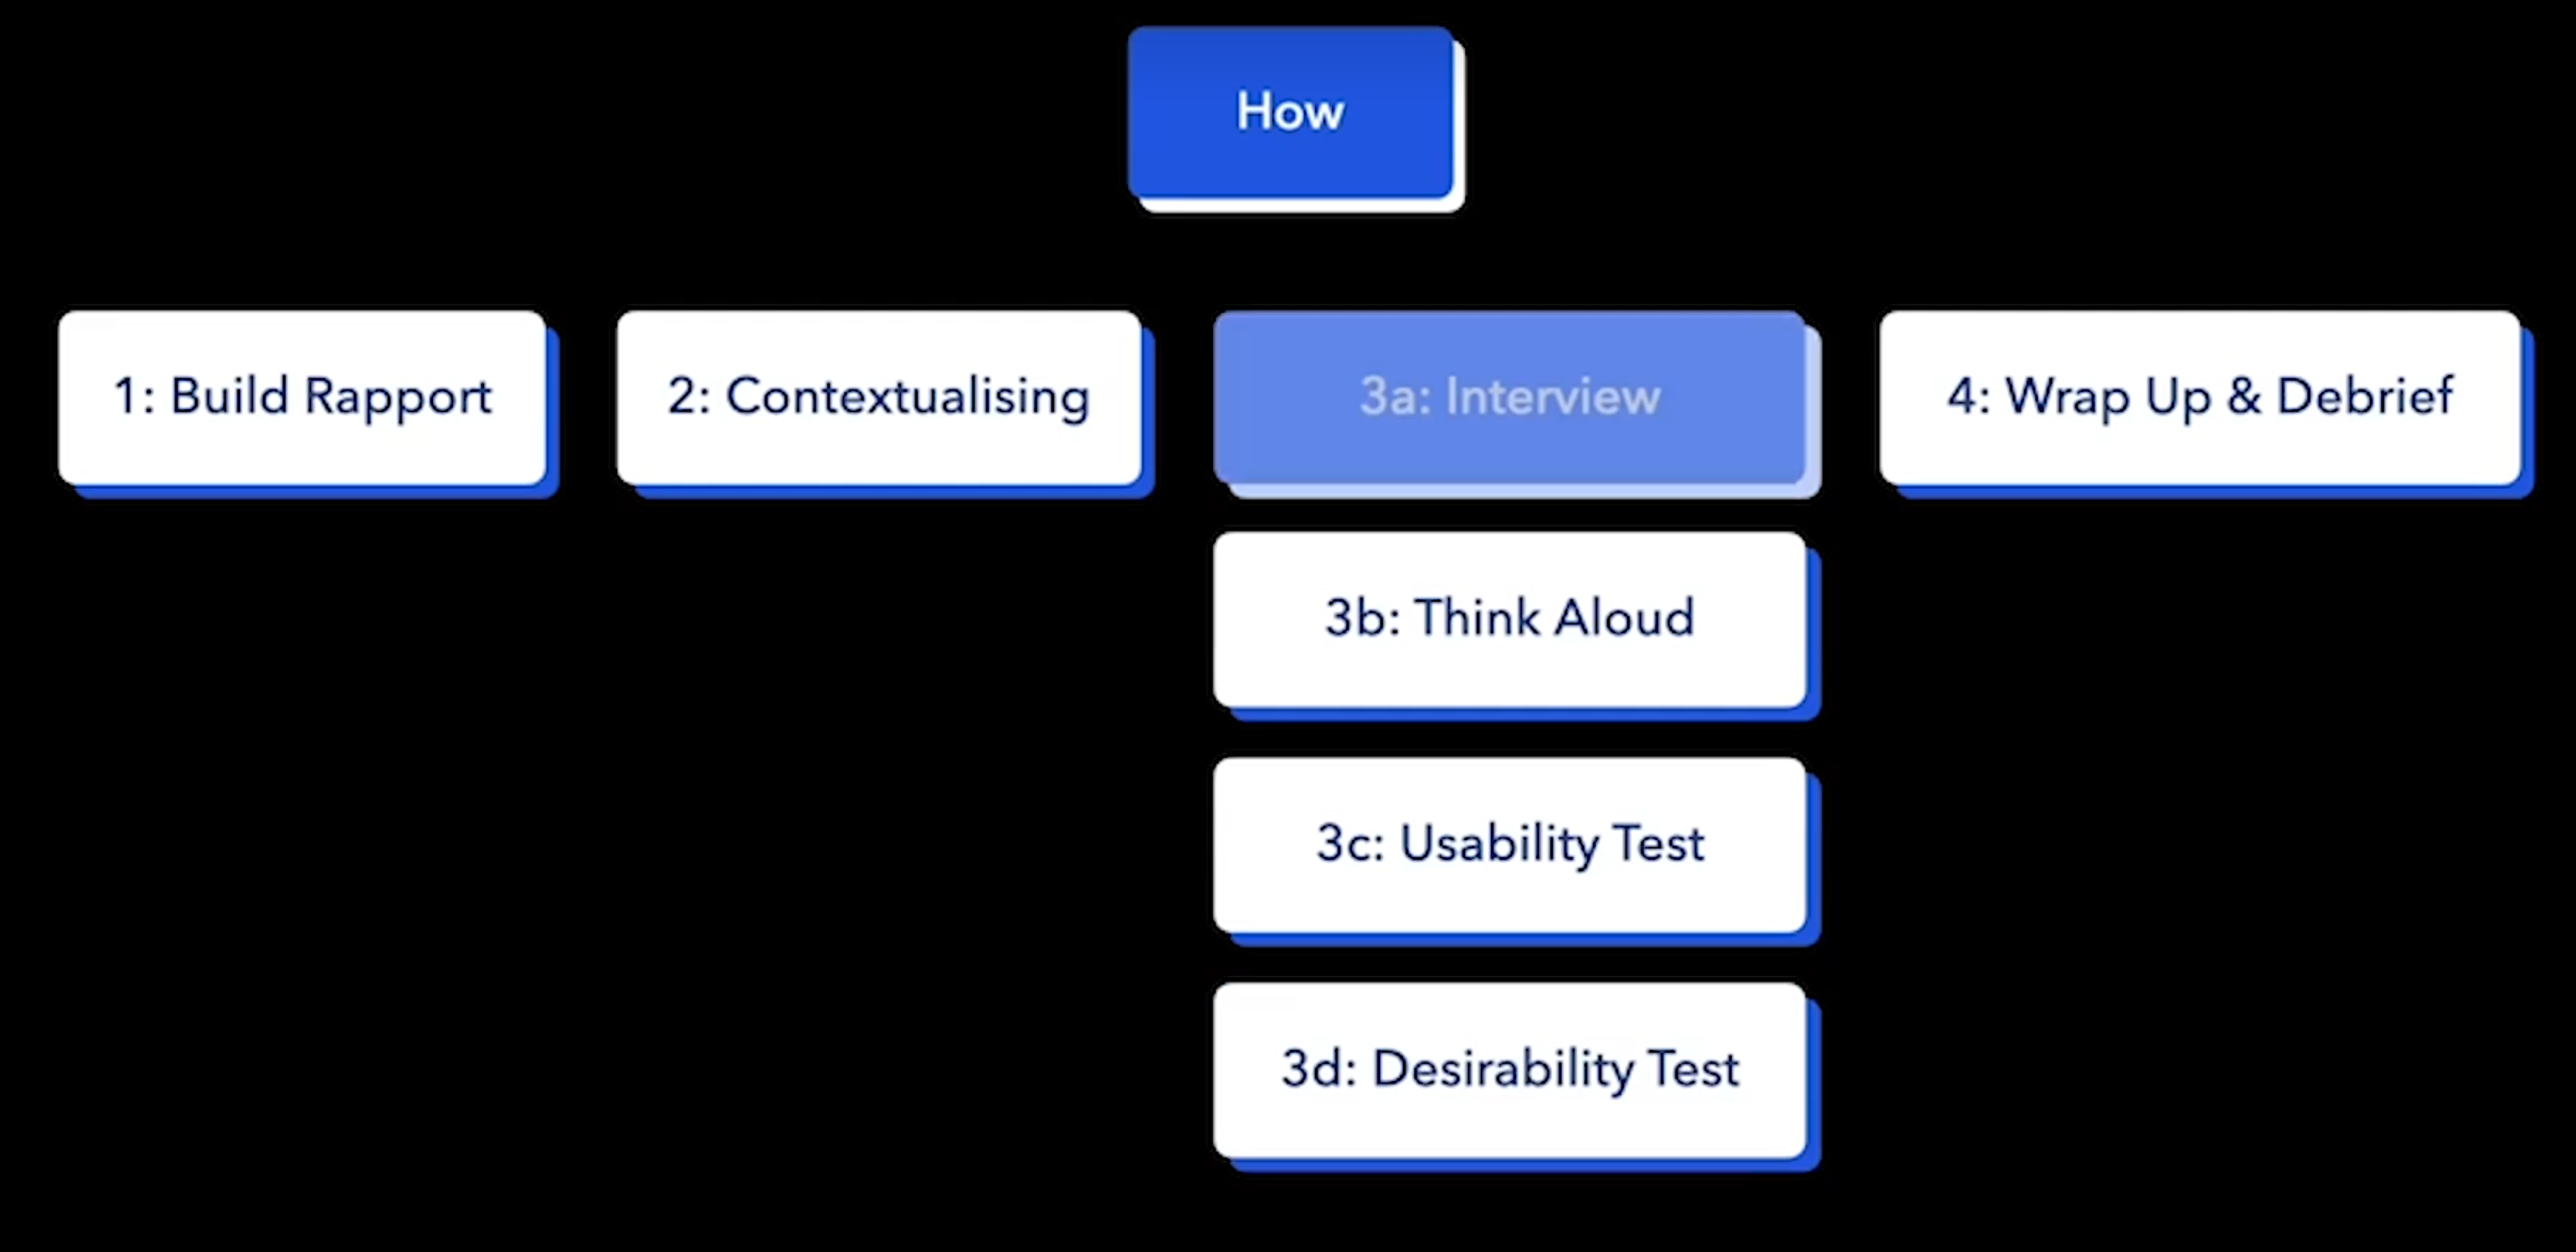
\includegraphics[width=0.5\linewidth]{images/evaluate-steps.png}
\end{figure}
Some tips
\begin{enumerate}
    \item Keep your users accurately informed.
    \item Seek permission, not forgiveness.
    \item Don't make promises you can't keep. Don't say some functions that are not available with your prototypes.
\end{enumerate}
\subsection{Practical Application of Evaluating with People}
The difference between this segment and the segment 2 is that, in this segment, we focus on testing the product through pre-planned user interactions and live feedback.
\subsection{Individual Learning Activity}
\begin{enumerate}
    \item Documentation: Take photos of the survey you conduct.
\end{enumerate}
\section{Individual Learning Activity}
\subsection{Develop Evaluation Strategy}
\begin{enumerate}
    \item \textbf{Describe your proposed solution}: My proposed solution is an efficient watering can with three key features
    \begin{itemize}
        \item Removable, Top-Mounted Water Tank: Easy to refill and large enough to supply sufficient water in one go. This is implemented by a plastic cup.
        \item Switch Mechanism: Controls water flow instantly between the tank and the pipes. This is implemented by creating a height difference between the top of the straw and the bottom of the cup.
        \item Three-Pipe System: Arranged in a triangular formation for stable and even water distribution. The pipes are implemented by straws.
    \end{itemize}
    \item \textbf{The most important thing to learn from this evaluation and why}: I mainly want to learn \textbf{whether my prototype is easy to use}, including the setup. a.k.a I want to know whether my prototype exhibits ``well-perceived affordances'' (This is what I have learned from the Intro Segment -- Norman Door!) I choose this focus mainly because of two reasons:
    \begin{itemize}
        \item I want to explore some fields I haven't touched during the prototype. And I feel this field can only be done by my user becuase I always think my prototype has "well-perceived affordances"
        \item I feel the ultimate goal of a product, or a prototype, should not only be to solve the user's problem, but also to be intuitive and easy to use. After all, we don't want to create something that is functional, but is actually a ``Norman Door'' right?
    \end{itemize}
    \item \textbf{Plan your evaluation}: How to conduct, where to conduct, which evaluation method to use, how would you allow participants to engage with your prototype, what questions would you ask? \\
    This is done on Excalidraw.
\end{enumerate}
\subsection{Synthesize your feedback}
\begin{enumerate}
    \item \textbf{Key Findings 1}: Lack of Clear Affordances Led to Misinterpretation. While setting up, my user inserted the pipes in a straight line instead of the intended triangular arrangement. This revealed a key insight: despite my prototype’s triangular design, it lacked well-perceived affordances, leading to confusion. I think the key reason is as follows
    \begin{itemize}
        \item Without a stable ``separation support'' structure, the three pipes aligned in a straight line when lifted, causing the user to misinterpret the intended setup.
    \end{itemize}
    \item \textbf{Next Steps 1}: To enhance my prototype’s **well-perceived affordances**, I plan to add a small triangle to separate the three pipes, ensuring clearer positioning. It will look like this:
    \item \textbf{Key Findings 2}: Stability Assumption Doesn’t Always Hold. During evaluation, I noticed my user's windowsill wasn’t level. This revealed a key insight: I had assumed a flat surface for plant placement, but that isn’t always the case.
    \item \textbf{Next Steps 2}: This observation sparked new insights for improving the prototype’s stability.
    \begin{itemize}
        \item Lowering the center of gravity (the traditional approach) improves stability.
        \item When the bottom contact surface isn’t level, this method becomes ineffective. In such cases, I believe a new approach is needed. I analyzed the system's imbalance and identified that the lack of tight connection between subsystems contributes to instability.
    \end{itemize}
    Therefore, my second approach is to strengthen the connections between subsystems using tape, which will enhance overall system stability. Here's my proposed solution to improve stability:
\end{enumerate}
\subsection{Documentation}
Should be photos of different steps, use words only to document the observations!
\subsection{Reflection}
From evaluating people, I learned that a good product should not only be functional (a.k.a solve user's problem), but also should be intuitive or easy to use (a.k.a exhibit ``well-perceived affordances''). After all, I believe  that we don't want to create something that works for us, but is difficult for others to use. (We should avoid designing some ``Norman Doors'').

For a product to be functional, prototyping is essential. For it to exhibit well-perceived affordances, evaluation is necessary.  For the first point, I have experienced the beauty of making prototypes work to solve my user's problem and improve it step by step. If so, why evaluation is needed for a prototype/product to exhibit ``well-perceived affordances''? Can we just look at our prototype and say, ``okay, my prototype is easy to use?''

I think the answer is ``No'' because prototyping itself cannot or is very hard to let me fully know whether my product/prototype exhibits ``well-perceived affordances'' or not. This is because when prototyping, we are thinking from a designer perspective. From my prototyping experience, I feel that I mainly focus on solving the problems (here is one golden rule from one of my Engineering courses, ``If it works, it works'' LOL). I think this makes it easy to overlook usability issues that may not seem like problems to me but can confuse my user. For example, during my evaluation, I have found that my user didn't know that the three pipes should be plugged into the soil in a triangle form. However, during my prototyping, I have never thought of that, because I only thought that triangle is the simplest and most stable shape. I feel this can be vividly describe using this scenario: as a designer, I develop an idea and pass it through a pipeline from the beginning, but at the end of the pipeline, the user’s perception of that idea may be entirely different from what I intended.

So how do we bridge this gap? I think this needs our product to exhibit ``well-perceived affordances''. However, achieving this from a designer’s perspective alone is difficult, which is why evaluation is crucial. Through evaluation, we observe and gather feedback from users, allowing us to refine our design to be more intuitive.

Why is evaluation effective in this regard? I think the key lies in shifting perspectives. In prototyping, our product is viewd from a designer perspective, which is that we look at our product. In evaluation, however, our product is viewed from a user's perspective. It's the users without prior knowledge of its design that interact with the product. They only know its intended purpose, which makes them the best judges of its intuitiveness. This shift reveals usability issues we might never anticipate. For example, during my prototyping, I test everything on a flat ground level, but when I go to my user's house, I find that his room's windowsill is not flat! This creates a big problem for my original solution to solve the stability issue! Fortunately, by re-looking at my prototype and think about this issue, I gained some brand-new insights on how to improve a system's stability, which is covered in my ``synthesize the feedback'' slide.

To wrap up, as almost the last segment, I feel so excited that something I have learned from the ``Intro Segment'' (``well-perceived affordances'') can be used here. For me, this journey makes me feel like this design thinking course is like a closed loop. From Intro Segment's Norman Door, to Segment 1's ideation (idealize some methods to solve a problem), then to Segment 2's empathy (empathize with the user to find a problem), then to Segment 3's prototype (make some things to actually solve the problem) and finally to Segment 4's evaluation (evaluate to add ``well-perceived affordances''). The last step actually goes back to the first step! I think that is the beauty of design thinking, by going through the process and finding out that we are actually apply what we have learned from the lecture videos into the real-world life. This is really amazing to me!

\chapter{Design Thinking Journal}
\section{Lecture Videos}
\subsection{Design Thinking}
\begin{enumerate}
    \item Design Thinking is a creative approach to solve problems or enhance existing solutions. It trains you to think in a designerly way, which simply refers to innate your human ability to respond to the world around you creatively. (``To make is to create, to create is to be human'').
    \item When we reflect on what we've learned, we give ourselves a chance to look at things differently, make connections that weren't obvious before and draw provocative inferences that lead us towards creative solutions that show off our unique point of view.
\end{enumerate}
\subsection{Tips for Reflection}
From lecture videos
\begin{enumerate}
    \item \textbf{Identify Experience}: Recall the experience, Describe and Distill
    \item \textbf{Analyzing Experience}: What's significant, Analyze and Evaluate
    \item \textbf{Questioning existing experiences}: Reflect on your emotions, what do they tell you?
    \item \textbf{Planning for future experiences}: Follow up with actions, make it personal
\end{enumerate}
From my tutor's basecamp!
\begin{enumerate}
    \item \textbf{Tell an authentic story of key learning moments}
    \begin{itemize}
        \item Ensure that your narrative is \textbf{coherent, personal} and \textbf{authentic}.
        \item It's not always about your wins, your \textbf{struggles} are equally instructive.
    \end{itemize}
    \item \textbf{Show evidence}
    \begin{itemize}
        \item Ground your claims with anecdotes\footnote{Interesting short stories} or evidence from ILAs, TBWs, conversations with people around you or any past moment in the past 13 weeks. \textbf{A picture says a thousand words}.
    \end{itemize}
    \item \textbf{Make connections}
    \begin{itemize}
        \item How can you take the lessons you've learnt into your life/other areas
    \end{itemize}
    \item \textbf{Be action-biased}
    \begin{itemize}
        \item Given what you've learnt from the experience, what can you do to grow? To do better next time?
    \end{itemize}
    \item If DTJ is written in paragraphs, can think about
    \begin{itemize}
        \item What do you realise when you iterate and sketch
        \item What do you learn about the design process or creating a physical/digital solution
    \end{itemize}
    Categorize your thoughts, give it an insightful title!
    \item \textbf{Formatting}: 
    \begin{itemize}
        \item \underline{Underline} and \textbf{Bold} the title of the point you are writing about.
        \item Use paragraph and/or point form.
        \item \textbf{Highlight} key moments to flash out the experience
        \item \textbf{Make it easy for people to read}!
    \end{itemize}
\end{enumerate}
For each of the three phases
\begin{enumerate}
    \item \textbf{Discovery Phase \& Development Phase}:
    \begin{itemize}
        \item Find a format that works for you (storyboarding, scrapbook,etc)
        \item Focus on \textbf{1 key moment} and your takeaway from it, then flash out that story
        \item Why was it pivotal for you? How do you see this moment as a way to solve problems?
    \end{itemize}
    \item \textbf{My Proposed Solution}:
    \begin{itemize}
        \item Where is your proposed solution right now? Where do you hope it should be?
        \item What are the next steps to take it to the next level?
        \begin{itemize}
            \item Do you want to collaborate with a community partner to bring this idea to life?
            \item Or would you prefer to conduct more market research to ensure there is a need for it?
        \end{itemize}
    \end{itemize}
\end{enumerate}
\begin{figure}
    \centering
    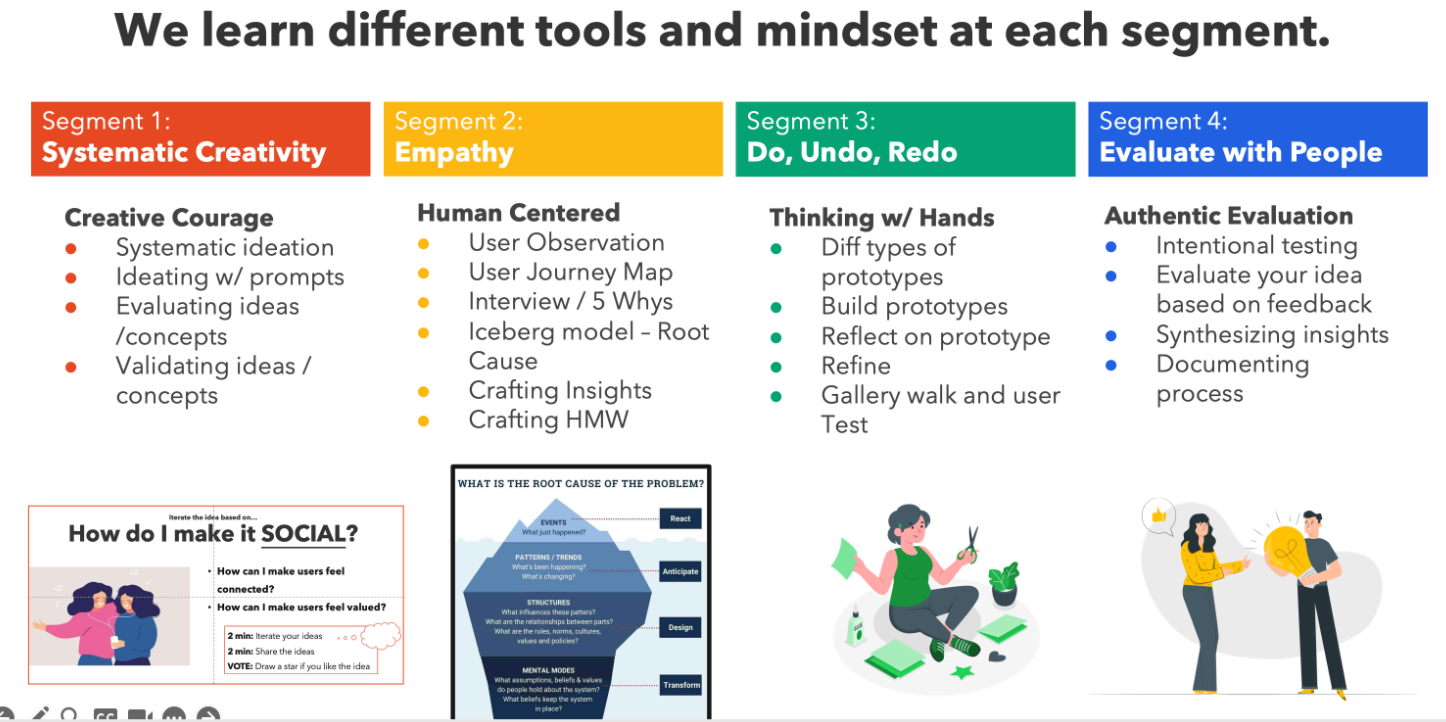
\includegraphics[width=0.75\linewidth]{images/dtj-reference.png}
    \caption{Each Tools we've learned from the ILAs}
    \label{fig:dtj-reference}
\end{figure}

\subsection{DTJ Rubrics}
\begin{enumerate}
    \item Insight and tacit connections made through one's learning show `point of view'.
    \item Not only look back at the experience, but also question in a positive manner, with the intention to improve the way one does things in the future.
\end{enumerate}
\end{document}
